\begin{figure}[h]
    \centering
    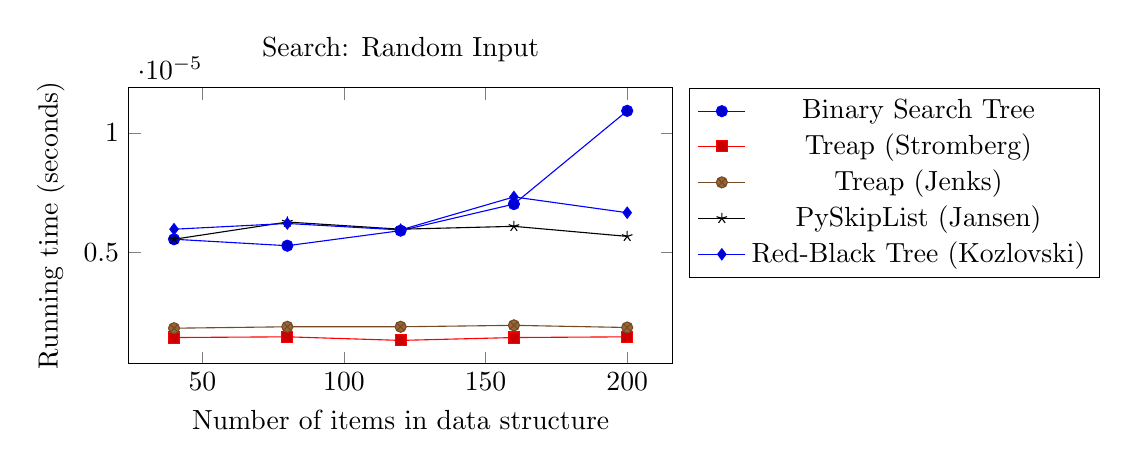
\begin{tikzpicture}
        \begin{axis}[
            xlabel={Number of items in data structure},
            ylabel={Running time (seconds)},
            title={Search: Random Input},
            width=0.7\textwidth,
            height=2in,
            legend pos=outer north east
        ]
		\addplot coordinates {
			(40, 5.541626196228777e-06)
			(80, 5.270568393153652e-06)
			(120, 5.903036600332645e-06)
			(160, 7.0173853463140205e-06)
			(200, 1.0932664724086494e-05)
		};
		\addplot coordinates {
			(40, 1.4155240827318226e-06)
			(80, 1.445641616407145e-06)
			(120, 1.295053948033309e-06)
			(160, 1.4155240827345984e-06)
			(200, 1.445641616407145e-06)
		};
		\addplot coordinates {
			(40, 1.8070520205082374e-06)
			(80, 1.8672870878616576e-06)
			(120, 1.8672870878616576e-06)
			(160, 1.927522155209527e-06)
			(200, 1.8371695541835597e-06)
		};
		\addplot coordinates {
			(40, 5.541626196231553e-06)
			(80, 6.264447004433737e-06)
			(120, 5.96327166768329e-06)
			(160, 6.083741802384579e-06)
			(200, 5.662096330930066e-06)
		};
		\addplot coordinates {
			(40, 5.96327166768329e-06)
			(80, 6.2042119370830925e-06)
			(120, 5.933154134007967e-06)
			(160, 7.318560683064468e-06)
			(200, 6.655974942212927e-06)
		};
        \legend{Binary Search Tree, Treap (Stromberg), Treap (Jenks), PySkipList (Jansen), Red-Black Tree (Kozlovski)}
        \end{axis}
    \end{tikzpicture}
    \caption{Average of 10 operations, benchmarked every 40, starting at 40.}
\end{figure}